\documentclass[12pt,a4paper]{article}
\usepackage[utf8]{inputenc}
\usepackage[T1]{fontenc}
\usepackage[margin=2.5cm]{geometry}
\usepackage{xcolor}
\usepackage{setspace}
\usepackage{array}
\usepackage{colortbl}
\usepackage{graphicx}
\usepackage{tocloft}
\usepackage{hyperref}
\usepackage{float}

\hypersetup{
    colorlinks=true,
    linkcolor=blue,
    urlcolor=blue
}

%==============================
% CONFIGURACIÓN GENERAL
%==============================
\setlength{\parindent}{1.5em}
\onehalfspacing
\setlength{\cftbeforesecskip}{6pt}
\renewcommand{\contentsname}{Índice}

%==============================
% COLORES
%==============================
\definecolor{azulnoche}{RGB}{0,40,90}
\definecolor{celesteclaro}{RGB}{224,240,255}
\definecolor{grisclaro}{RGB}{245,245,245}
\definecolor{darkgreen}{rgb}{0.533, 0.486, 0.184}
\definecolor{golden}{RGB}{197,160,89}
\definecolor{goldford}{RGB}{143,113,54}
\definecolor{rojo}{RGB}{166,25,46}

%==============================
% NUMERACIÓN PERSONALIZADA
%==============================
\renewcommand{\thesection}{\Roman{section}}
\renewcommand{\thesubsection}{\arabic{section}.\arabic{subsection}}
\renewcommand{\thesubsubsection}{\thesubsection.\arabic{subsubsection}}

\begin{document}

% ==============================
% PORTADA
% ==============================
\begin{titlepage}
\centering
{\normalsize\textbf{"Año de la Esperanza y el Fortalecimiento de la Democracia"}}\\
\vspace{0.5cm}

{\color{golden}\bfseries\large UNIVERSIDAD NACIONAL MAYOR DE SAN MARCOS}\\
\vspace{0.1cm}
{\color{golden}\large\textbf{(Universidad del Perú, Decana de América)}}\\
\vspace{0.5cm}


\includegraphics[width=0.35\textwidth]{UNMSM_coatofarms_seal.svg.png}\\
\vspace{0.5cm}

{\color{goldford}\scshape\Large Facultad de Ingeniería de Sistemas e Informática\\}
\vspace{0.5cm}

\color{rojo}\hrule height 0.3mm\vspace{0.2cm}
{\color{rojo}\Large\bfseries MONOGRAFÍA: COMPUTACIÓN CUÁNTICA\vspace{0.56cm}}\\
\color{rojo}\hrule height 0.3mm\vspace{0.5cm}

{\color{rojo}\Large\textbf{Curso:}}\\
{\color{goldford}\Large Introducción a la Computación}\\

\vspace{0.3cm}
{\color{rojo}\Large\textbf{Docente:}}\\
{\color{goldford}\Large Uscuchagua Flores, Gelber Christian}\\

\vspace{0.3cm}
{\color{rojo}\Large\textbf{Integrantes:}}\\
{\color{goldford}\large 
Angeles, Gian Franco \\
Eneque Roca, Jair Stefano \\
Espinal Bazan, Sebastián Andres \\
Fernandez Curas, Christian Jair \\
}

\vspace{1.5cm}
{\color{goldford}\Large\textbf{LIMA - PERÚ}}\\
{\color{goldford}\Large\textbf{2026}}\\
\end{titlepage}

% ==============================
% ÍNDICE
% ==============================
\tableofcontents
\newpage

% ==============================
% I. INTRODUCCIÓN
% ==============================
\section{Introducción}

% ==============================
% II. DESARROLLO
% ==============================
\section{Desarrollo}

%-------------------------------------------------
\subsection{Capítulo I. Principios y Fundamentos de la Computación Cuántica}

\subsubsection{Evolución de la computación clásica a la computación cuántica}
La computación clásica, cuyas bases lógicas y teóricas fueron formalizadas por Alan Turing y otros investigadores en la década de 1930, se fundamenta en bits binarios que toman valores discretos de 0 o 1 y en operaciones lógicas ejecutadas por circuitos electrónicos basados en el álgebra de Boole. 
Durante décadas, este paradigma guió el desarrollo informático bajo la premisa subyacente de que la computación es un proceso físico sujeto a leyes termodinámicas y naturales. No obstante, las limitaciones intrínsecas de los sistemas convencionales para simular sistemas de la física cuántica de manera eficiente se hicieron evidentes hacia finales del siglo XX.\\

El surgimiento formal de la computación cuántica se atribuye a una célebre conferencia dictada por Richard Feynman en 1982, el cual imaginó teóricamente una máquina que pudiera imitar y simular de forma fidedigna la mecánica cuántica utilizando los propios principios de la física cuántica.
Además, esta visión fue formalizada por David Deutsch en 1985 con el concepto de la Máquina de Turing Cuántica, demostrando que tales dispositivos podrían realizar tareas inalcanzables para los sistemas clásicos.
Por lo cual, el impulso científico global hacia la construcción de este hardware se aceleró críticamente en 1994, cuando Peter Shor demostró matemáticamente que una computadora cuántica podría factorizar números enteros de forma eficiente, comprometiendo de manera directa los criptosistemas de clave pública modernos como la encriptación RSA.\\

\begin{figure}[htbp]
    \raggedright
    {\bfseries Figura 1}\\
    \textit{Línea de tiempo de la evolución histórica de la computación cuántica}\\
    \vspace{0.3cm}
    \centering
    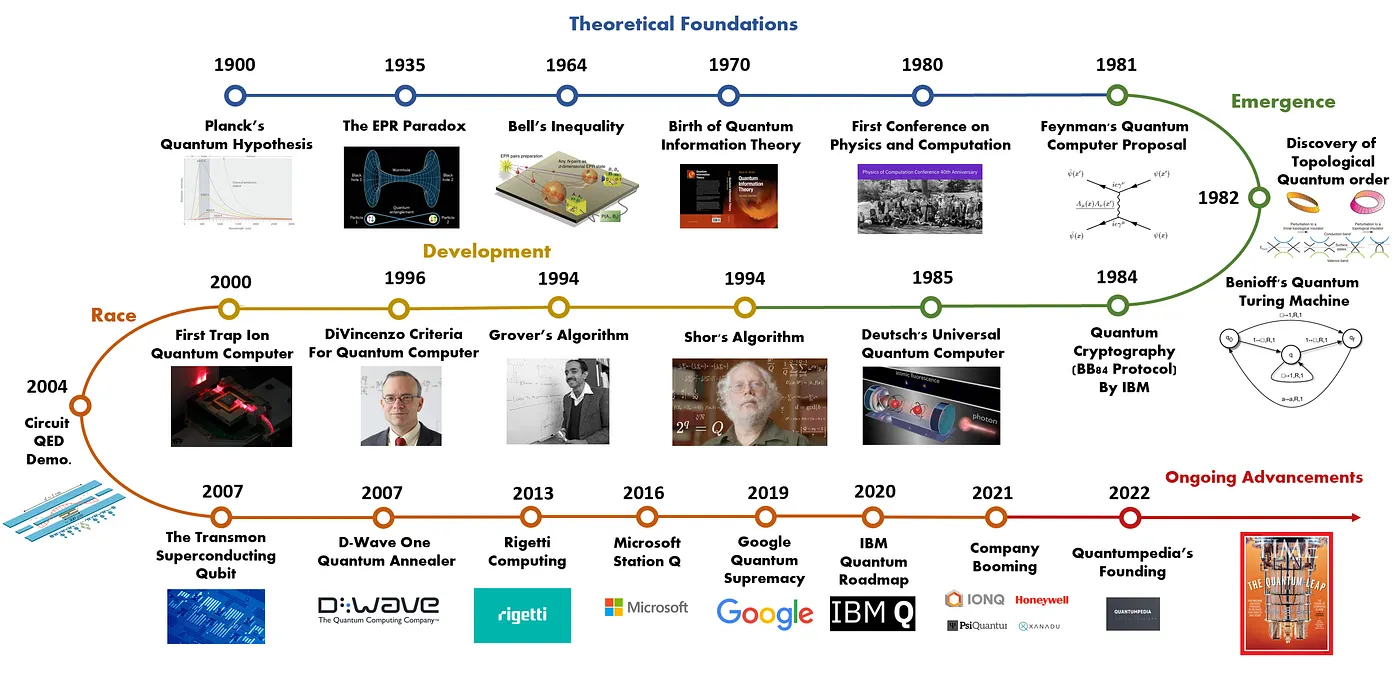
\includegraphics[width=0.85\textwidth]{linea_tiempo.png}\\
    \vspace{0.3cm}
    \raggedright\small
    \textit{Nota.} Adaptado de \textit{A Brief History of Quantum Computing}, por Quantumpedia, 2020 (https://quantumpedia.uk/a-brief-history-of-quantum-computing-e0bbd05893d0).
\end{figure}

Como se puede apreciar en la Figura 1, la transición desde los fundamentos computacionales clásicos hasta la consolidación de la teoría cuántica no fue un evento aislado, sino una concatenación de hitos conceptuales. La cronología resalta cómo los desafíos teóricos planteados inicialmente por Feynman y Deutsch encontraron una aplicación crítica y disruptiva con el algoritmo de Shor. Este recorrido histórico demuestra que el paso del bit al qubit no solo representó una mejora en la velocidad de procesamiento, sino un cambio radical en las leyes físicas aplicadas a la teoría de la información, sentando las bases tecnológicas del hardware contemporáneo.

\subsubsection{El qubit como unidad fundamental de información}
Mientras que la arquitectura clásica procesa la información mediante el bit convencional, la computación cuántica introduce el bit cuántico o \textit{qubit} como su bloque elemental y unidad fundamental de información. Físicamente, un qubit se define como un sistema cuántico direccionable de dos niveles de energía.\\

Matemáticamente, el estado puro de un qubit se modela como un vector de estado que reside dentro de un espacio de Hilbert complejo bidimensional. Haciendo uso de la notación bra-ket de Dirac, el estado general de un qubit, denotado como $|\psi\rangle$, se expresa formalmente a través de la combinación lineal de sus estados de base computacional, $|0\rangle$ y $|1\rangle$, definida por la ecuación:

\begin{equation}
    |\psi\rangle = \alpha |0\rangle + \beta |1\rangle
\end{equation}

donde $\alpha$ y $\beta$ son amplitudes de probabilidad complejas que cumplen la condición de normalización $|\alpha|^2 + |\beta|^2 = 1$. Esta propiedad permite que $n$ qubits representen simultáneamente $2^n$ valores posibles, expandiendo el espacio computacional (espacio de Hilbert) de manera exponencial. Físicamente, los qubits pueden implementarse mediante el espín de un electrón, la polarización de un fotón o estados de carga en circuitos superconductores.\\
\begin{figure}[H]
    \raggedright
    {\bfseries Figura 2}\\
    \textit{Representación geométrica de un qubit en la esfera de Bloch}\\
    \vspace{0.3cm}
    \centering
    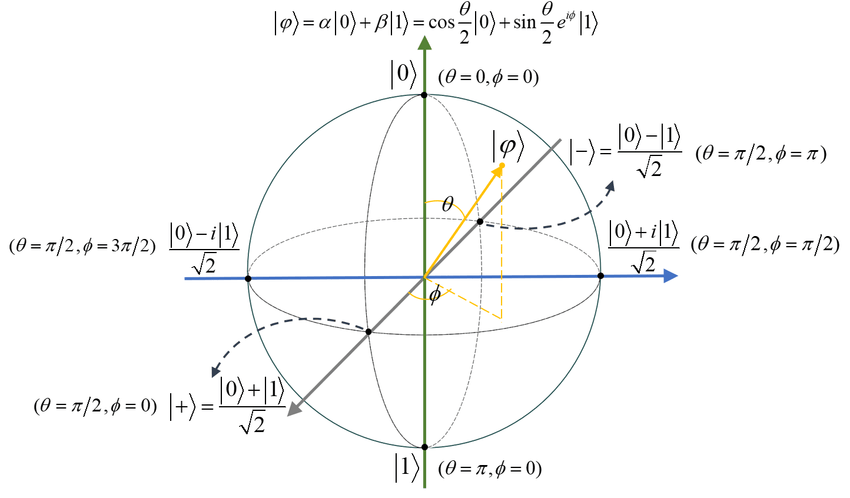
\includegraphics[width=0.45\textwidth]{Bloch.png}\\
    \vspace{0.3cm}
    \raggedright\small
    \textit{Nota.} Tomado de \textit{Efficient Quantum Secure Vector Dominance and Its Applications in Computational Geometry}, por W. Liu, B. Su y F. Sun, 2025, \textit{IEEE Transactions on Computers}, 74(6), pp. 2129–2143 (https://doi.org/10.1109/TC.2025.3557968).
\end{figure}

Tal y como se puede visualizar en la Figura 2, la esfera de Bloch proporciona una abstracción geométrica indispensable para visualizar el estado de un qubit aislado dentro de un espacio tridimensional. Mientras que un bit clásico está limitado a los polos norte o sur de esta esfera (representando estrictamente los estados discretos $|0\rangle$ y $|1\rangle$), un qubit puede localizarse en cualquier punto sobre la superficie de la esfera. Los ángulos colatitud y longitud de la superficie parametrizan las amplitudes complejas $\alpha$ y $\beta$, lo que evidencia de forma visual cómo el principio de superposición permite la coexistencia e infinitas combinaciones de estados. Esta propiedad geométrica es fundamental para el diseño de algoritmos, ya que las operaciones lógicas cuánticas equivalen analíticamente a rotaciones controladas alrededor de los ejes de este espacio esférico.

\subsubsection{Principios de la mecánica cuántica aplicados a la computación}
La ventaja de procesamiento radical que exhibe el paradigma cuántico sobre los enfoques digitales clásicos radica en la explotación directa de los postulados fundamentales de la mecánica cuántica. Los principios esenciales integrados en el procesamiento de información son los siguientes:

\begin{itemize}
    \item \textbf{Superposición cuántica:} Es la propiedad física que faculta a un sistema (como el qubit) para coexistir simultáneamente en múltiples estados combinados ($|0\rangle$ y $|1\rangle$) con amplitudes de probabilidad definidas, en lugar de verse confinado de forma exclusiva a una única alternativa binaria rígida.
    \item \textbf{Entrelazamiento cuántico:} Fenómeno físico en el cual los estados cuánticos de dos o más partículas u objetos se vinculan de tal manera que el estado de uno de ellos no puede describirse de forma independiente del otro, sin importar la distancia física que los separe. El entrelazamiento genera correlaciones no locales masivas y un procesamiento en paralelo inalcanzable por medios convencionales.
    \item \textbf{Interferencia:} Se utiliza en los algoritmos para amplificar las amplitudes de probabilidad de los resultados correctos y cancelar mediante interferencia destructiva los resultados erróneos.
\end{itemize} 

Un aspecto crítico es la medición, la cual colapsa el estado de superposición en un resultado determinista (0 o 1), destruyendo la información cuántica previa. Además, el teorema de no clonación prohíbe la creación de copias idénticas de un estado cuántico desconocido, lo que diferencia radicalmente la gestión de errores cuánticos de la clásica (Nasser, 2025, p.5).

\subsubsection{Puertas lógicas y circuitos cuánticos}
Las operaciones en computación cuántica se ejecutan mediante \textbf{puertas lógicas cuánticas}, que son transformaciones unitarias aplicadas a los qubits. A diferencia de las puertas clásicas, las cuánticas son inherentemente reversibles.\\

Entre las puertas fundamentales se encuentran:
\begin{itemize}
    \item \textbf{Puerta Hadamard (H):} Crea superposición a partir de estados base.
    \item \textbf{Puertas de Pauli (X, Y, Z):} Realizan rotaciones en la esfera de Bloch, como la puerta X que actúa como un \textit{NOT} cuántico.
    \item \textbf{Puerta CNOT (Controlled-NOT):} Una puerta de dos qubits esencial para generar entrelazamiento.
\end{itemize}

Un circuito cuántico es una secuencia de estas puertas aplicadas a un estado inicial para realizar un cálculo específico. Asimismo, se ha demostrado que conjuntos pequeños de estas puertas son universales, lo que significa que cualquier operación unitaria puede aproximarse con precisión arbitraria mediante una secuencia finita de ellas (Madanan et al., 2023).

\subsubsection{Tecnologías de hardware cuántico}
La materialización física de un ordenador cuántico escalable requiere de un sistema tecnológico capaz de satisfacer rigurosamente los denominados criterios de DiVincenzo formalizados en el año 2000. 
Dichos criterios exigen cinco directrices fundamentales para el procesamiento: (a) un sistema físico escalable con qubits bien caracterizados , (b) la capacidad de inicializar los estados de los qubits , (c) tiempos largos de coherencia cuántica , (d) un conjunto universal de compuertas cuánticas , y (e) la capacidad de realizar mediciones específicas en qubits individuales (He-Liang Huang et al., 2020).

\subsubsection{Estado actual del hardware cuántico}

%-------------------------------------------------
\subsection{Capítulo II.}

\subsubsection{}


%-------------------------------------------------
\subsection{Capítulo III.}

\subsubsection{}


%-------------------------------------------------
\subsection{Capítulo IV. }

\subsubsection{}


% ==============================
% III. CONCLUSIONES
% ==============================
\section{Conclusiones}

% ==============================
% IV. REFERENCIAS
% ==============================
\section{Referencias}

\end{document}

```